\section{Project Results}

% \subsection{Upgrade Dependencies}
% 
% \begin{frame}[c]
%     From Django 2 to Django 3 \\
%     (Django 4 released during the project, has been decided to go to 3 in production first) \\
%     Now requires \mintinline{python}{DEFAULT_AUTO_FIELD = "django.db.models.AutoField"}
% \end{frame}

\subsection{Proper Logging}

\begin{frame}[c]{Changes to Logging}
    \large
    \begin{itemize}[<+(1)->]
        \item Used to be done in inconsistent format over individual \mintinline{python}{print} statements
        \item Good to get overview of Codebase and touch many files
        \item Now: Properly defined Logging levels (debug, info, warn, error, critical)
        \item Now: Log messages are sent to console, syslog and saved in a file locally
        \item Now: file and console formatting differs (timestamps, colors, ...)
        \item Now: Rotating files: Keep last five days, overwrite after
    \end{itemize}
\end{frame}

\pic{Logging Now: Example}{33}


\subsection{Automatically Generate Documentation}

\begin{frame}[c]{Why attempt automatic documentation?} 
    \large
    Situation:
    \begin{itemize}[<+(1)->]
        \item Still only rudimentary grasp on Codebase
        \item Especially on available routes, endpoints, internal dependencies
    \end{itemize}
    \pause
    Expectations:
    \begin{itemize}[<+(1)->]
        \item Automatic, Complete, Up-to-date Overview
        \item Creation of a frequently used reference
        \item Provides a documentation pipeline and default
    \end{itemize}
\end{frame}

\begin{frame}[c]{Automatically Generate Documentation}
    \begin{multicols}{2}
        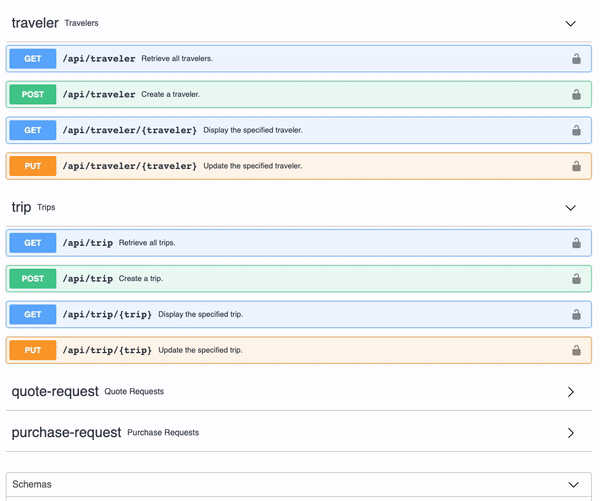
\includegraphics[width=0.5\textwidth]{swagger} \\
        (Success from different Project) \\
        \large
        Failed, because:
        \begin{itemize}[<+(1)->]
            \item Autogeneration usually used to generate documentation for {\em JSON endpoints}
            % \item Few comments to generate documentation from
            \item 'Primitive' Views lacking important information for automatic generation
        \end{itemize}
        Was worth a try.
    \end{multicols}
\end{frame}


\subsection{What Research is the Storage used for?}

\begin{frame}[c]{What Research is the Storage used for?}
    \begin{multicols}{2}
        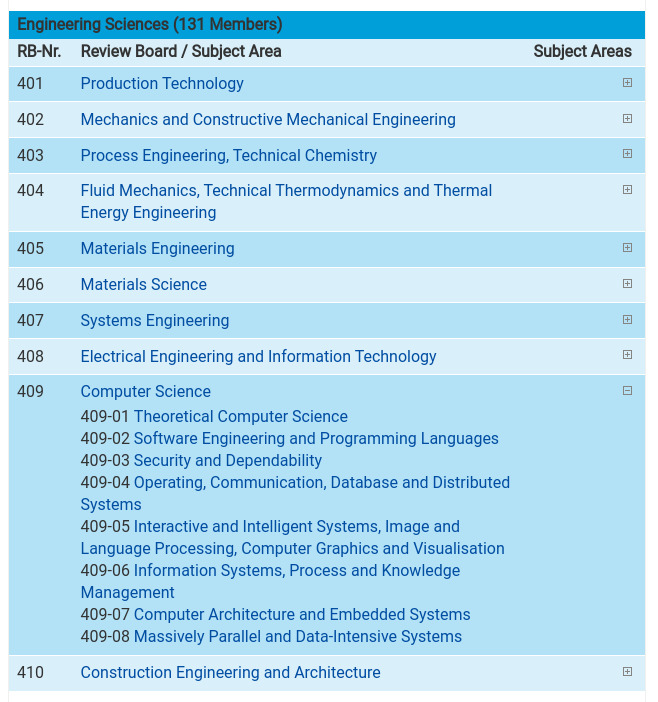
\includegraphics[width=0.5\textwidth]{Selection_032} \\
        \begin{itemize}[<+(1)->]
            \item For reporting and analysis Purposes
            \item We want to know more about our users
            \item This includes affiliation of research projects
            \item Good existing classification from 'Deutsche~Forschungsgesellschaft'
        \end{itemize}
    \end{multicols}
\end{frame}

\pic{Selection of DFG Subject Area upon Project Creation}{10}

\begin{frame}[c]{Selection of DFG Discipline}
    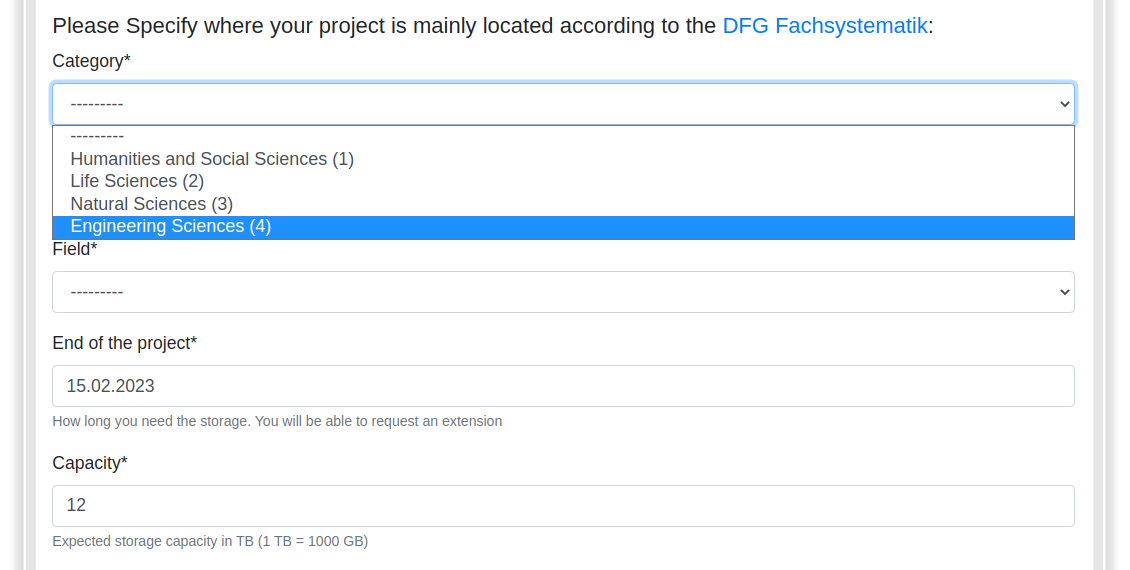
\includegraphics[width=\textwidth]{select_category}
\end{frame}
\begin{frame}[c]{Selection of DFG Subject Area without Board}
    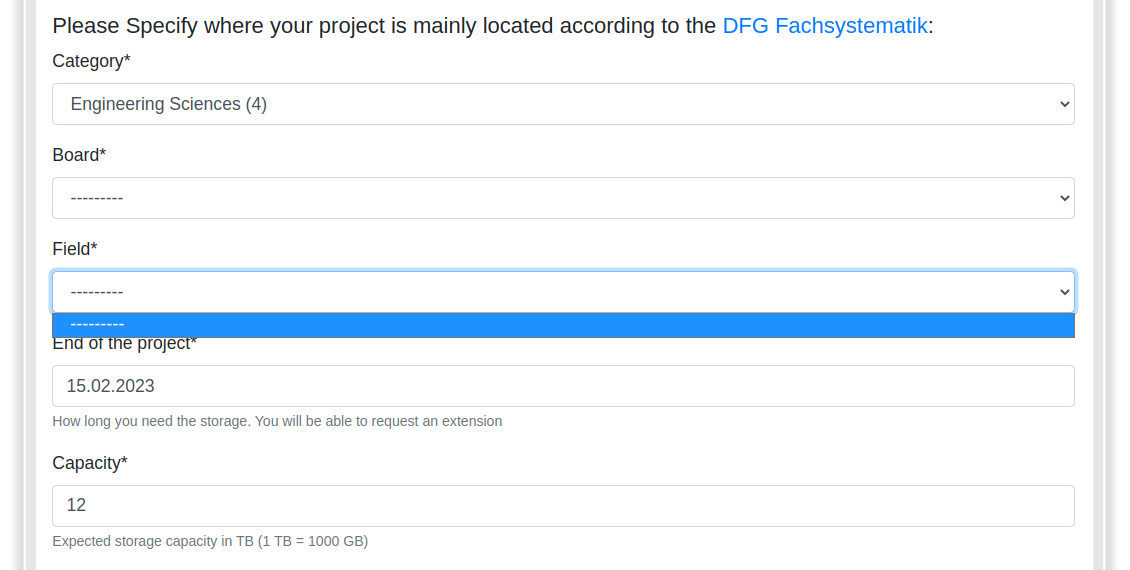
\includegraphics[width=\textwidth]{select_field1}
\end{frame}
\begin{frame}[c]{Selection of DFG Review Board}
    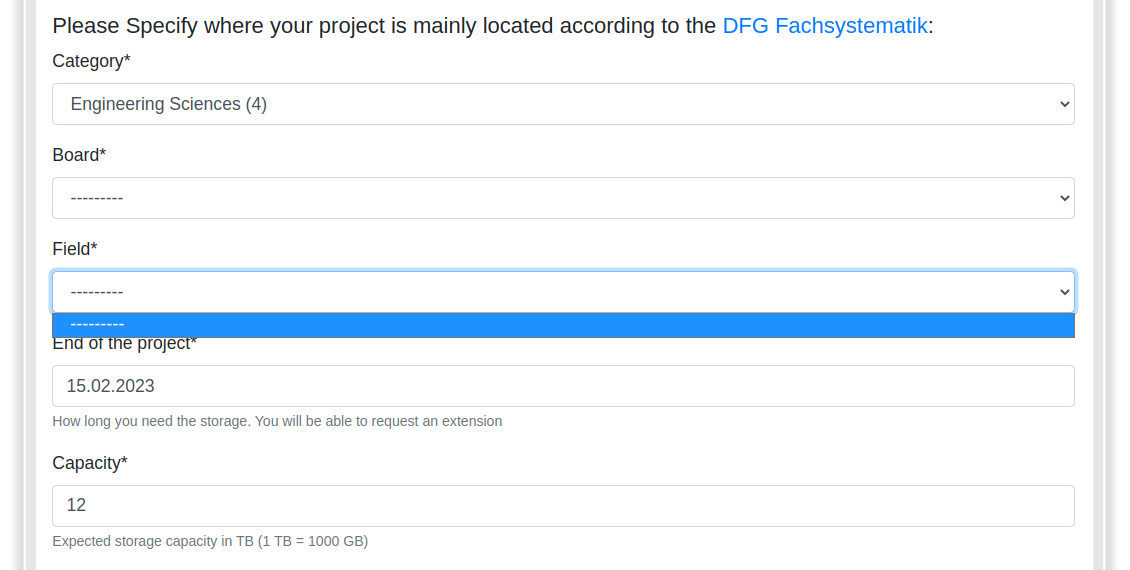
\includegraphics[width=\textwidth]{select_field1}
\end{frame}
\begin{frame}[c]{Selection of DFG Subject Area}
    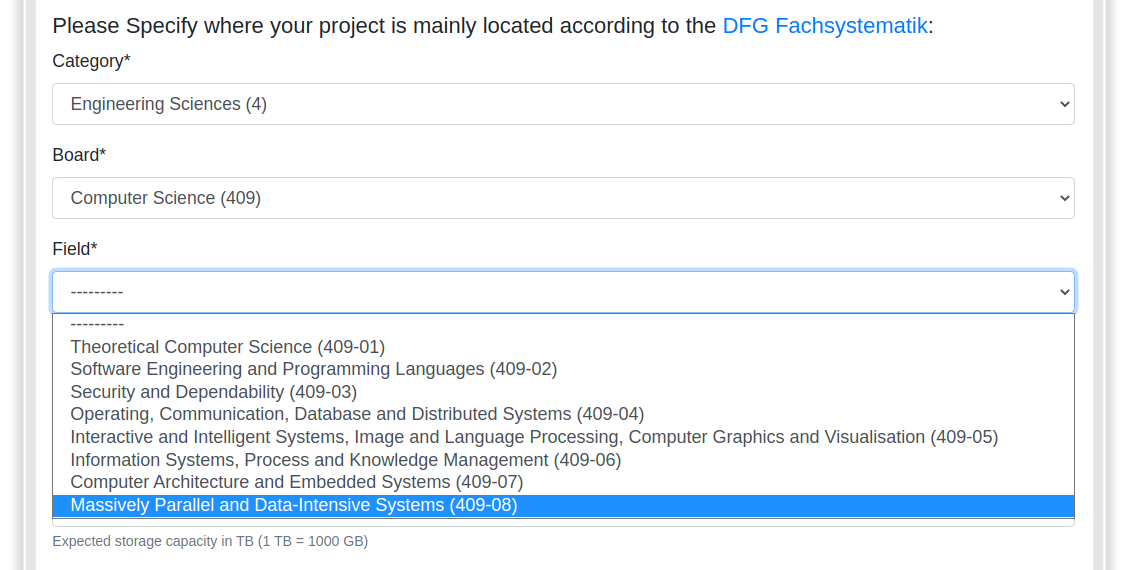
\includegraphics[width=\textwidth]{select_field2}
\end{frame}


\begin{frame}[c,fragile]{Website: Requesting Fields for Boards}
    \footnotesize
    \inputminted[linenos=true]{javascript}{code/board_request.js}
\end{frame}


\begin{frame}[c,fragile]{Backend: answering with available Fields}
\footnotesize
    \begin{minted}[linenos]{python}
## urls.py
path('ajax/fields/', views.view_science_fields, name="ajax_load_fields"),

## views.py
def view_science_fields(request):
    b_pk = request.GET.get('board')  # we get the pk of the selected board
    if b_pk:  # select available Fields from this Board
        fields = Science_Field.objects.filter(board__pk=b_pk) 
        return render(request, 'dropdown_list_options.html',
                      {'options': fields}
                    )
    return render(request, 'dropdown_list_options.html',
                  {'options': Science_Field.objects.none()}
                )
\end{minted}
\end{frame}

\begin{frame}[c]{Visualisation}
    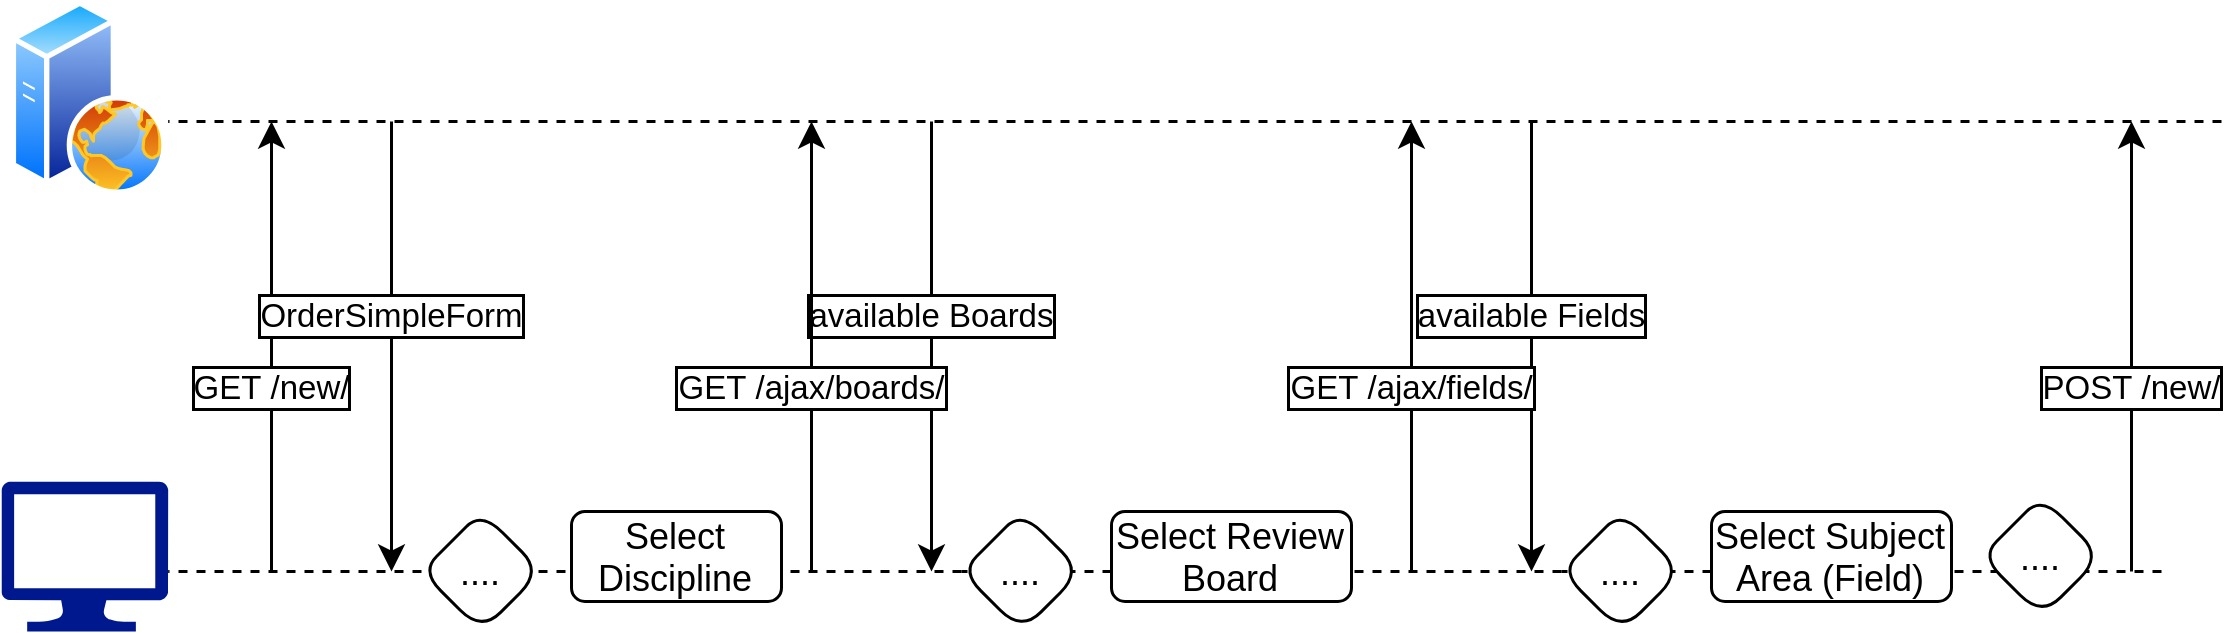
\includegraphics[width=\textwidth]{board_requests}
\end{frame}

\subsection{Diff CSV to DFG Schema in Database}

\begin{frame}[c]{The DFG schema changes frequently}
    \large
    \begin{itemize}[<+(1)->]
        \item The DFG schema changes every four years
        \item It was last changed in 2020
        \item So it'll change again in two years
        \item Not clear how much (probably not a whole lot)
    \end{itemize}
    \pause
    So I implemented a command to compare any csv to what is currently in the
    database: \mintinline{bash}{manage.py dfg_schema_diff}
\end{frame}


% \begin{frame}[fragile]{Usage of \texttt{dfg_schema_diff}}
\begin{frame}[fragile]{Usage of \texttt{dfg\_schema\_diff}}
    \scriptsize
\begin{verbatim}
usage: manage.py dfg_schema_diff [-h] [--locale LOCALE] [--columns COLUMNS]
                     ...
                     FILE

Show difference from given file schema to DFG schema in database. By default,
ignores the now deprecated hierarchy level 1. ...

positional arguments:
  FILE                  Path to dfg_systematic.csv

options:
  -h, --help            show this help message and exit
  --locale LOCALE       Set the language of the name column to select. Can correctly select
                        both '<locale>' and 'prefLabel@<locale>' columns. (Default: 'en')
  --columns COLUMNS     Dictionary mapping columns (numbers) to expected values "level" (in
                        the hierarchy, category: 0, deprecated/ignored: 1, board: 2, field:
                        3), "notation" (e.g. 101-27), and locale translations, e.g. "en"
                        (double quotes are important!). Defaults to auto.
  ...                   ...
\end{verbatim}
\end{frame}

% \subsection{Rename Models}
% 
% \begin{frame}[c]
%     % Order -> LSDFProject
%     % PersonOrder -> ProjectRole
%     % ...
%     Worked quite well, generated some migrations
% \end{frame}

% \subsection{Attempt to rename entire App}
% 
% \begin{frame}[c]
%     Failed, ultimately unclear why, requires deep django/database knowledge.
% \end{frame}


\subsection{Attempt to properly modularize PersonForm}
\begin{frame}[c]
    \scriptsize
    \inputminted[linenos]{python}{code/personform.py}
\end{frame}



%     \begin{frame}[c]{PersonForm and Views}
%     So I created a ModelForm for Person.
%     And a Personformset.
%     And startet to integrate it in the OrderSimpleForm
%     \end{frame}

\begin{frame}[c]{Intermediate Results}
    \begin{multicols}{2}
        \tiny
        \inputminted[linenos]{python}{code/personforms.py}
        \normalsize
        \begin{itemize}[<+(1)->]
            \item Abstraction to one dedicated PersonForm
            \item PersonFormSet can have arbitrarily many Persons (was only five)
            \item Simplifies implementation in View
            \item Difficult to propagate ValidationErrors properly
            \item Would have deleted about 300 lines of boilerplate
            % \item Problem: A view is supposed to show only a single Form
                % \item Problem: Took a long time to implement
        \end{itemize}
    \end{multicols}
\end{frame}

\begin{frame}[c]{Reasons for Failure}
    % Managed to get quite far, very good (deep) learning example, and absolutely
    % possible. just requires some more time than expected.
    % Nags me that it's not modular yet. Some day.
    \large
    \begin{itemize}[<+(1)->]
        \item Nesting of \mintinline{python}{Forms} is \textbf{not} supported (\mintinline{python}{owner} within \mintinline{python}{OrderSimpleForm})
        \item Particularly with the many assumptions and automated parts of \mintinline{python}{ModelForm}s
        % \item Need to manually call all steps from other \mintinline{python}{ModelForm}
        \item Manually register fields for \mintinline{python}{ValidationErrors}
        \item Manually put in values for Validation (from \mintinline{python}{PersonFormSet})
        \item Manually take values out to save new Models
    \end{itemize}
    \pause
    Nothing impossible, but requires a lot of intricate details to get right.
    \pause
    We decided to instead implement something else.
\end{frame}


\subsection{Extension Requests}

\begin{frame}[c]{Motivation}
    It happens frequently that a project needs more space than initially
    requested, or isn't done by the time their timeframe runs out (initial
    timeframe was 4 Years). In these cases, timeframe and capacity can be
    extended manually by an admin. To automate/improve this process, we
    implemented it directly.
\end{frame}


\pic{Timeframe Extension Request View}{19}
\pic{Capacity Extension Request View}{20}
\pic{Filled out Capacity Extension}{21}
\pic{Extension System Message}{22}
\pic{System Message showing Extension Approval}{28}
\pic{Increased Capacity from User View}{29}

\begin{frame}[c]{Routing for Timeframe Requests}
    \large
    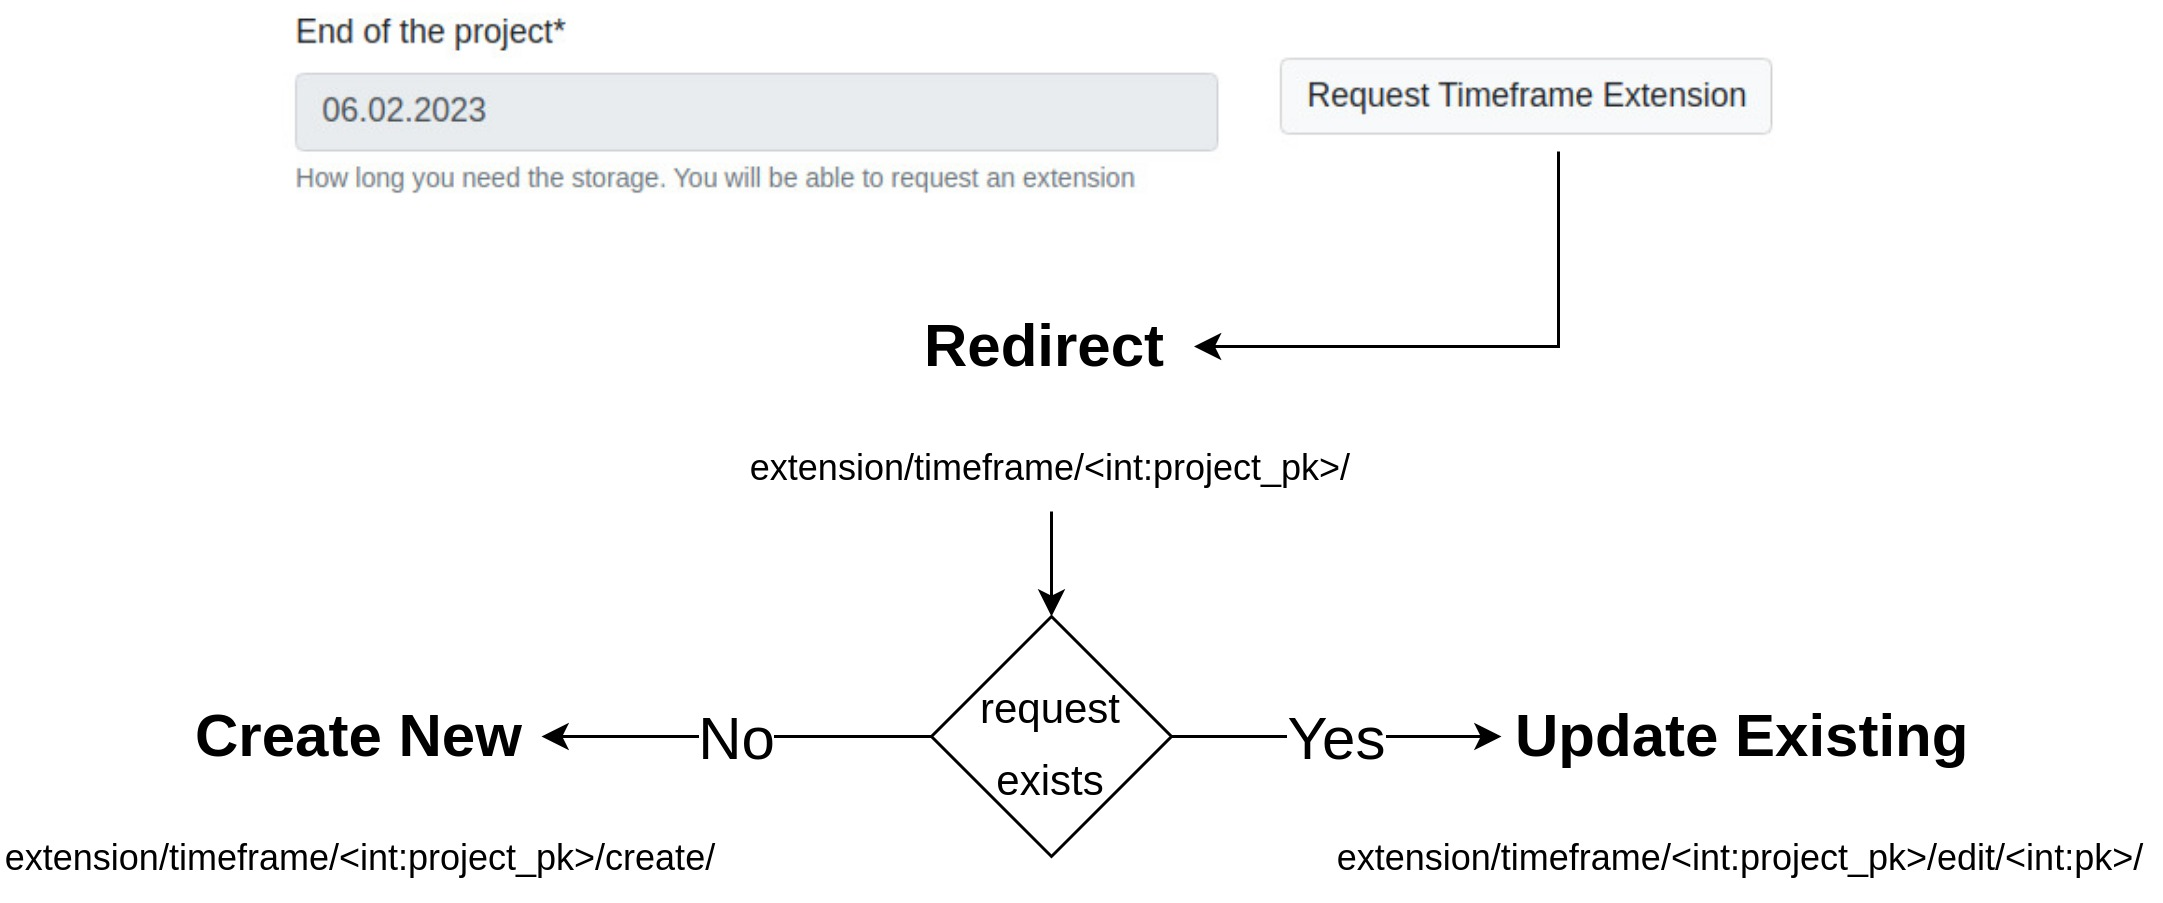
\includegraphics[width=\textwidth]{timeframe_routing}
\end{frame}
